\documentclass{rapportECL}
\usepackage{lipsum}
\usepackage{svg}
\usepackage{algorithm}
\usepackage{algorithmic}
\usepackage{longtable}
\usepackage{subcaption} 
\usepackage[utf8]{inputenc}
\usepackage{ragged2e}   


\title{Rapport ECL - Template} %Titre du fichier

\begin{document}

%----------- Informations du rapport ---------

\titre{Implémentation d'Algorithmes pour les Systèmes d'Argumentation Abstraits} %Titre du fichier .pdf
\UE{Représentation des Connaissances et Raisonnement} %Nom de la UE
\sujet{ Introduction à l’Argumentation - Projet} %Nom du sujet

\enseignant{Elise \textsc{Bonzon}} %Nom de l'enseignant

\eleves{Hugo \textsc{Convert} \\
		Kiswendsida \textsc{OUEDRAOGO} } %Nom des élèves

%----------- Initialisation -------------------
        
\fairemarges %Afficher les marges
\fairepagedegarde %Créer la page de garde
\tabledematieres %Créer la table de matières

%------------ Corps du rapport ----------------
\begin{abstract}
	Ce rapport présente le travail réalisé dans le cadre du développement d’un outil informatique dédié à la résolution de problèmes 
	dans le domaine des systèmes d’argumentation abstraits. Nous avons commencé par une exploration approfondie des algorithmes de 
	calcul des extensions complètes et stables, en nous appuyant sur des travaux de recherche issus de la littérature scientifique 
	sur l’argumentation. Ces algorithmes ont été décrits en détail, accompagnés d’explications sur leurs mécanismes et les structures 
	de données utilisées pour leur implémentation.

    Grâce à ces algorithmes, nous avons pu répondre aux problématiques posées dans le sujet du projet, telles que la détermination 
	des extensions d’un système d’argumentation donné et l’évaluation de l’appartenance d’un argument à une extension.

    En complément, nous avons développé une interface graphique conviviale permettant de visualiser les systèmes d’argumentation, 
	leurs arguments, et les relations entre eux, offrant ainsi une meilleure interaction utilisateur et facilitant l’analyse des 
	résultats. Ce rapport détaille les méthodologies employées, les choix techniques effectués et les résultats obtenus, illustrant 
	ainsi notre contribution à la mise en œuvre pratique des concepts théoriques de l’argumentation.
\end{abstract}

\newpage % Crée une nouvelle page après l'abstract


\section{Introduction} 
Pour la réalisation de ce projet, une revue de littérature s’est naturellement imposée. Parmi les ressources pertinentes, nous avons trouvé plusieurs travaux particulièrement intéressants. 

En premier lieu, nous avons étudié le cours d'Élise Bonzon sur l'argumentation computationnelle \cite{a}, notamment , qui nous a servi de base pour comprendre les concepts fondamentaux. 
Nous avons également exploré l'article \textit{An Introduction to Argumentation Semantics} \cite{b}, qui propose des définitions assez approfondies des différentes sémantiques de l'argumentation. 
Enfin, l’étude des algorithmes pour les sémantiques d'argumentation, présentée dans \textit{Algorithms for Argumentation Semantics: Labeling Attacks as a Generalization of Labeling Arguments} \cite{c}, 
nous a permis d’approfondir nos connaissances sur les algorithmes utilisés dans ce domaine et ainsi implémenter la solution du projet présent. 

Cette exploration nous a permis de définir les objectifs du projet, présentés dans la section suivante.

\section{Objectifs et fonctionnalités attendues du projet}
Ce projet vise à développer un outil capable de résoudre des problèmes spécifiques liés aux systèmes d'argumentation abstraits (AF). 
Un système d'argumentation est défini par un ensemble d'arguments (A) et une relation d'attaque (R) entre ces arguments. 
L'objectif est de fournir une solution capable d’identifier les extensions complètes et stables, et évaluer l’appartenance 
d’un argument à ces extensions selon des critères crédibles ou sceptiques.

Le programme lit un système d'argumentation à partir d'un fichier texte formaté, analyse les données, et produit des résultats conformes selon la sémantique utilisée. 


Le projet propose également une interface visuelle  representant les arguments, leurs relations sous forme de graphes et ainsi que les résultats des analyses pour faciliter l’interaction utilisateur et l’interprétation des résultats.

\section{Algorithmes et structures de données} 


\subsection{Algorithmes}
Les algorithmes utilisés pour l'implémentation de ce projet sont spécifiquement ceux dédiés à l'énumération des extensions complètes 
et stables. Ces algorithmes sont issus des travaux présentés dans l'article 
\textit{"Algorithms for Argumentation Semantics: Labeling Attacks as a Generalization of Labeling Arguments"}  \cite{c}.
Pour les deux algorithmes qui seront présentés dessous, tournera autour autour de l'utilisation d'étiquettes qui sont IN, OUT,  {MUST\_OUT}, BLANK et UNDEC.
{MUST\_OUT} et BLANK n'ayant pas été abordé en cours, sont en effet ici des détails d'implémentation.


L'étiquette \textbf{IN} identifie les arguments qui pourraient appartenir à  l'extension recherchée. L'étiquette \textbf{OUT} 
identifie un argument qui est attaqué par un argument \textbf{IN}. L'étiquette \textbf{BLANK} est attribuée à tout argument non 
traité dont l'étiquette finale n'est pas encore déterminée. L'étiquette \textbf{ {MUST\_OUT}} identifie les arguments qui attaquent des 
arguments \textbf{IN}. Enfin, l'étiquette \textbf{UNDEC} désigne les arguments qui pourraient ne pas être inclus dans  l'extension, car ils pourraient ne pas être défendus par un argument \textbf{IN}.


\begin{itemize}
    \item Énumération des extensions stables.
    
	L'algorithme ci-dessous identifie toutes les extensions stables d’un AF $(A, R)$ \cite{c} (p. 642). %\cite{ref}  
	On remarque l'absence d'utilisation du label \textbf{UNDEC}. La sémantique du label \textbf{MUST\_OUT} peut être interprétée comme celle 
	d'un \textbf{UNDEC} qui attaque un argument étiqueté \(\textbf{IN}\). 
	Cependant, dans une labellisation visant à identifier une extension stable, aucun argument ne devrait rester étiqueté \textbf{UNDEC} à 
	la fin. 

	C'est pourquoi le label \textbf{MUST\_OUT} est utilisé à la ligne 34 pour désigner les arguments susceptibles d'évoluer 
	vers \textbf{OUT} à la fin de la labellisation. Ainsi, un ensemble d'arguments \( S \), étiqueté \(\textbf{IN}\), est 
	considéré comme stable uniquement s'il n'existe aucun argument étiqueté \textbf{MUST\_OUT} à l'issue de la labellisation.

	\begin{algorithm}
		\caption{Enumerating all stable extensions of an AF $(A, R)$}
		\begin{algorithmic}[1]
			\STATE $Lab : A \to \{IN, OUT,  MUST\_OUT, BLANK\}$; $Lab \gets \emptyset$
			\FORALL{$x \in A$}
				\STATE $Lab \gets Lab \cup \{(x, BLANK)\}$
			\ENDFOR
			\STATE $Estable \subseteq 2^A$; $Estable \gets \emptyset$
			\STATE \textbf{call} find-stable-extensions($Lab$)
			\STATE \textbf{report} $Estable$ is the set of all stable extensions
			\STATE \textbf{procedure} find-stable-extensions($Lab$)
			\WHILE{there exists $y \in A$ such that $Lab(y) = BLANK$}
				\IF{there exists $y$ such that $Lab(y) = BLANK$ and $\forall z \in \{y\}^- : Lab(z) \in \{OUT,  MUST\_OUT\}$}
					\STATE select $y$ such that $Lab(y) = BLANK$
				\ELSE
					\STATE select $y$ such that $Lab(y) = BLANK$ and $\forall z : Lab(z) = BLANK$, 
					\STATE $\left| \{x : x \in {y}^+ \land Lab(x) \neq OUT \} \right| \geq \left| \{x : x \in {z}^+ \land Lab(x) \neq OUT \} \right|$
				\ENDIF
				\STATE $Lab' \gets Lab$
				\STATE $Lab'(y) \gets IN$
				\FORALL{$z \in {y}^+$}
					\STATE $Lab'(z) \gets OUT$
				\ENDFOR
				\FORALL{$z \in {y}^-$}
					\IF{$Lab'(z) = BLANK$}
						\STATE $Lab'(z) \gets  MUST\_OUT$
					\ENDIF
					\IF{for all $w \in {z}^-$, $Lab'(w) \neq BLANK$}
						\STATE $Lab(y) \gets  MUST\_OUT$
					\ENDIF
				\ENDFOR
				\STATE \textbf{goto} line 7
				\STATE \textbf{call} find-stable-extensions($Lab'$)
				\IF{there exists $z \in {y}^-$ such that $Lab(z) = BLANK$}
					\STATE $Lab(y) \gets  MUST\_OUT$
				\ELSE
					\STATE $Lab \gets Lab'$
				\ENDIF
				\IF{for all $x$, $Lab(x) \neq  MUST\_OUT$}
					\STATE $S \gets \{x : Lab(x) = IN\}$
					\STATE $Estable \gets Estable \cup \{S\}$
				\ENDIF
			\ENDWHILE
		\end{algorithmic}
	\end{algorithm}
	\begin{quote}
$(y, z) \in R$ signifie que $y$ attaque $z$ (ou que $z$ est attaqué par $y$).  
On note $\{y\}^-$ l'ensemble des arguments qui attaquent $y$,  
et $\{y\}^+$ l'ensemble des arguments attaqués par $y$.  
	\end{quote}	


Le processus commence par l'initialisation des arguments avec un label  {BLANK}, signifiant qu'aucun argument n'a encore été catégorisé. 
Ensuite, l'algorithme cherche à trouver toutes les extensions stables possibles en étiquetant les arguments de manière appropriée. 
Tant qu'il existe des arguments non étiquetés, l'algorithme sélectionne un argument \( y \) avec un label  {BLANK}. 
Le critère de sélection dépend de la situation : si l'argument \( y \) n'a pas d'attaquants non étiquetés (c'est-à-dire que tous ses attaquants ont déjà été étiquetés comme  {OUT} ou ), il est selectionné, 
ce qui signifie qu'il fait partie de l'extension.  Dans le cas contraire, l'algorithme choisit un argument \( y \) de manière à maximiser le nombre d'arguments attaqués par \( y \) (\( {y}^+ \)) qui ne sont pas encore étiquetés \(  {OUT} \).


Une copie complète de l'état des labels est effectuée pour la propagation des étiquettes (Lab' <- Lab)


Une fois un argument sélectionné et étiqueté  {IN}, l'algorithme modifie les labels des arguments attaqués par \( y \). Tous les arguments attaqués par \( y \) (les voisins de \( y \) dans l'ensemble \( \{y\}^+ \)) reçoivent le label  {OUT}, indiquant qu'ils sont exclus de l'extension. 
Les arguments voisins attaquant \( y \) \(\in\) \( \{y\}^- \) mais qui ne sont pas encore étiquetés ( {BLANK}) reçoivent le label  { MUST\_OUT}, signifiant qu'ils doivent être exclus de manière forcée et ne peuvent pas faire partie de l'extension. 

Si tous les attaquants \( \{z\}^- \) d'un argument \( z \) sont déjà étiquetés autre que ( {BLANK}), cela entraîne la mise à jour du label de \( y \) en  { MUST\_OUT} l'état des labels original, 
car l'argument \( y \) devient ainsi incompatible avec l'extension en cours et on execute un retour anticipé au début de la boucle while.

Une fois que les labels ont été modifiés, l'algorithme procède à une exploration récursive en appelant à nouveau la procédure pour tester de nouvelles configurations. 


On s'assure qu'il n'existe aucun argument \( z \) dans l'ensemble \( \{y\}^- \) qui soit étiqueté \(  {BLANK} \) dans l'état \( Lab \). Si tel est le cas, l'argument \( y \) est étiqueté \(  {MUST\_OUT} \). Sinon, l'état \( Lab \) est mis à jour pour être égal à l'état tampon \( Lab' \).

Si tous les arguments attaqués par \( y \) ont des labels autres que  { MUST\_OUT}, l'extension est considérée comme stable et l'ensemble des arguments étiquetés  {IN} est ajouté à l'ensemble des extensions stables.

l'exécution du bloc suivant l'appel récursif est mise dans la pile d'exécution, et elle sera traitée après tous les appels récursifs.

\newpage

\item Énumération des extensions complètes.
L'algorithme ci dessous de identifie toutes les extensions complètes d’un AF (A,R)  \cite{c} (p.644).

\begin{algorithm}
    \caption{Enumerating all complete extensions of an AF $(A, R)$}
    \begin{algorithmic}[1]
        \STATE $Lab : A \to \{\text{IN}, \text{OUT}, \text{MUST\_OUT}, \text{UNDEC}, \text{BLANK}\}$; $Lab \gets \emptyset$
        \FORALL{$x \in A$}
            \STATE $Lab \gets Lab \cup \{(x, \text{BLANK})\}$
        \ENDFOR
        \STATE $E_{\text{complete}} \subseteq 2^A$; $E_{\text{complete}} \gets \emptyset$
        \STATE \textbf{call} find-complete-extensions($Lab$)
        \STATE \textbf{report} $E_{\text{complete}}$ is the set of all complete extensions
        \STATE \textbf{procedure} find-complete-extensions($Lab$)
        \IF{there exists $y \in A$ such that $Lab(y) = \text{MUST\_OUT}$}
            \RETURN
        \ENDIF
        \IF{for all $x \in A$, $Lab(x) \in \{\text{UNDEC}, \text{BLANK}\} \implies \forall z \in \{x\}^-, Lab(z) = \text{OUT}$}
            \STATE $S \gets \{w \in A \mid Lab(w) = \text{IN}\}$
            \STATE $E_{\text{complete}} \gets E_{\text{complete}} \cup \{S\}$
        \ENDIF
        \WHILE{there exists $y \in A$ such that $Lab(y) = \text{BLANK}$}
            \IF{$\forall z \in \{y\}^-, Lab(z) \in \{\text{OUT}, \text{MUST\_OUT}\}$}
                \STATE select $y$ such that $Lab(y) = \text{BLANK}$
            \ELSE
                \STATE select $y$ such that $Lab(y) = \text{BLANK}$ and $\forall z : Lab(z) = \text{BLANK}$,
                \STATE $\left| \{x \mid x \in {y}^+ \land Lab(x) \neq \text{OUT} \} \right| \geq \left| \{x \mid x \in {z}^+ \land Lab(x) \neq \text{OUT} \} \right|$
            \ENDIF
            \STATE $Lab' \gets Lab$
            \STATE $Lab'(y) \gets \text{IN}$
            \FORALL{$z \in {y}^+$}
                \STATE $Lab'(z) \gets \text{OUT}$
            \ENDFOR
            \FORALL{$z \in {y}^-$}
                \IF{$Lab'(z) \in \{\text{UNDEC}, \text{BLANK}\}$}
                    \STATE $Lab'(z) \gets \text{MUST\_OUT}$
                \ENDIF
                \IF{for all $w \in {z}^-, Lab'(w) \neq \text{BLANK}$}
                    \STATE $Lab(y) \gets \text{UNDEC}$
                \ENDIF
            \ENDFOR
            \STATE \textbf{goto} line 7
            \STATE \textbf{call} find-complete-extensions($Lab'$)
            \IF{there exists $z \in {y}^-$ such that $Lab(z) \in \{\text{BLANK}, \text{UNDEC}\}$}
                \STATE $Lab(y) \gets \text{UNDEC}$
            \ELSE
                \STATE $Lab \gets Lab'$
            \ENDIF
        \ENDWHILE
    \end{algorithmic}
\end{algorithm}

 L'algorithme est repose sur le même principe que le préccédent avec quelques petits changements pour satisfaire les conditions d'extension stable.
 On part toujours sur la base d'arguments tous etiquettés à blanc;  le critère de selection d'argument pour la propagation des labels restant le même.
 On constate l'utilisation du label UNDEC ici lorsqu'une incompatibilité est levé en lieu et place de MUST\_OUT dans l'algorithm 1.
 
 on détermine si un ensemble \( S \) (les éléments dont le label est \( \text{IN} \)) est une extension complète en vérifiant 
 deux conditions. 

 	\begin{enumerate}
		\item Tout d'abord, garantir qu' aucun élément \( x \) de \( A \) n'est marqué 
		comme \( \text{MUST OUT} \).
		\item Ensuite, on vérifie qu'il n'existe pas un élément \( z \) 
		qui reste indéterminé (\( \text{UNDEC} \) ou \( \text{BLANK} \)) et qui aurait tous ses attaquants (les éléments de \( \{z\}^- \)) déjà marqués comme \( \text{OUT} \).
	\end{enumerate}

\end{itemize}

\newpage

\subsection{structures de données}

La manipulation des données dans le projet repose essentiellement sur l’utilisation de listes et de dictionnaires pour la représentation des arguments et des relations d’attaque.

\begin{itemize}
    \item Les arguments sont stockés dans une liste ou un ensemble. Par exemple : 
    \[
    {arguments = \{"A", "B", "C"\}}
    \]
    où \( A \), \( B \) et \( C \) représentent les arguments.

    \item Les attaques sont représentées par un dictionnaire, chaque clé correspondant à un argument et la valeur étant l’ensemble des arguments qu’il attaque. Par exemple :
    \[
    {attacks = \{"A": \{"B", "C"\}, "B": \{"C"\}\}}
    \]
    Ici, \( A \) attaque \( B \) et \( C \), tandis que \( B \) attaque \( C \).
\end{itemize}


\section{Implémentation et tests}

\subsection{Implémentation}

La proposition de solution a été faite \textbf{Python}. Nous avons choisi Python pour sa simplicité d'implémentation et sa flexibilité pour la manipulations des structures 
de données  telles que les listes et les dictionnaires que nous utilisons.

\subsubsection{Architecture}

L'architecture du projet repose sur l'utilisation de classes et de méthodes afin de faciliter le partage des données et des fonctions entre différents composants répartis sur plusieurs fichiers. Les principales parties de l'architecture sont décrites ci-dessous :

\begin{itemize}
    \item \textbf{main.py} : Ce fichier sert de point d'entrée principal pour l'exécution de la solution. L'utilisateur peut lancer le programme en mode console avec les paramètres suivants :
    \begin{itemize}
        \item \texttt{-P} : pour spécifier la sémantique de calcul.
        \item \texttt{-f} : pour indiquer le fichier contenant l'Argumentation Framework (AF).
        \item \texttt{-a} : (optionnel) pour spécifier les arguments, en fonction de la sémantique choisie.
    \end{itemize}
    Ce fichier appelle les autres fichiers pour le traitement des données et l'exécution des algorithmes, parmi lesquels on a:

    \item \textbf{utilities.py} : Ce fichier contient des classes et des méthodes utilitaires, comme la classe \texttt{file\_reader}, qui permet de lire les fichiers contenant l'AF. Ces méthodes facilitent la gestion des fichiers et la manipulation des données avant leur traitement.

    \item \textbf{controller.py} : Ce fichier contient les méthodes responsables de la gestion des flux de données. Il fait appel aux méthodes de calcul spécifiques en fonction des paramètres fournis par l'utilisateur, en organisant et en contrôlant l'exécution des algorithmes.

    \item \textbf{computing\_methods.py} : Ce fichier contient l'implémentation des algorithmes d'énumération des extensions complètes et stables. Afin de garantir une bonne lisibilité du code, les parties répétitives dans les algorithmes ont été extraites et regroupées dans des méthodes uniques. Par exemple, la méthode \texttt{select\_argument} est utilisée pour sélectionner un argument dans les différents algorithmes afin de réduire la duplication du code.

    \item \textbf{af\_visualizer.py} : Ce fichier gère l'interface graphique de l'application. Il est basé sur les mêmes méthodes des fichiers précédemment mentionnés, permettant une interaction visuelle avec l'utilisateur pour soumettre des fichiers et afficher les résultats sous une forme graphique.
\end{itemize}

\subsection{Tests et validation}

Pour vérifier l'exactitude de notre implémentation des algorithmes d'énumération des extensions stables et complètes, nous avons réalisé des tests sur plusieurs frameworks argumentatifs. Les commandes utilisées, ainsi que les résultats correspondants (captures de la console et de l'interface graphique), sont présentés ci-dessous.

\vspace{0.5cm}
\noindent


\begin{longtable}{|p{7cm}|p{7cm}|}
	\hline
	\textbf{Commande exécutée} & \textbf{Résultats (console et interface graphique)} \\ 
	\hline
	\endfirsthead
	\hline
	\textbf{Commande exécutée} & \textbf{Résultats (console et interface graphique)} \\ 
	\hline
	\endhead
	\hline
	\endfoot
	

	\texttt{python main.py -p SE-CO -f ./tests/af1.apx} & 
	\begin{minipage}{\linewidth}
		\centering
		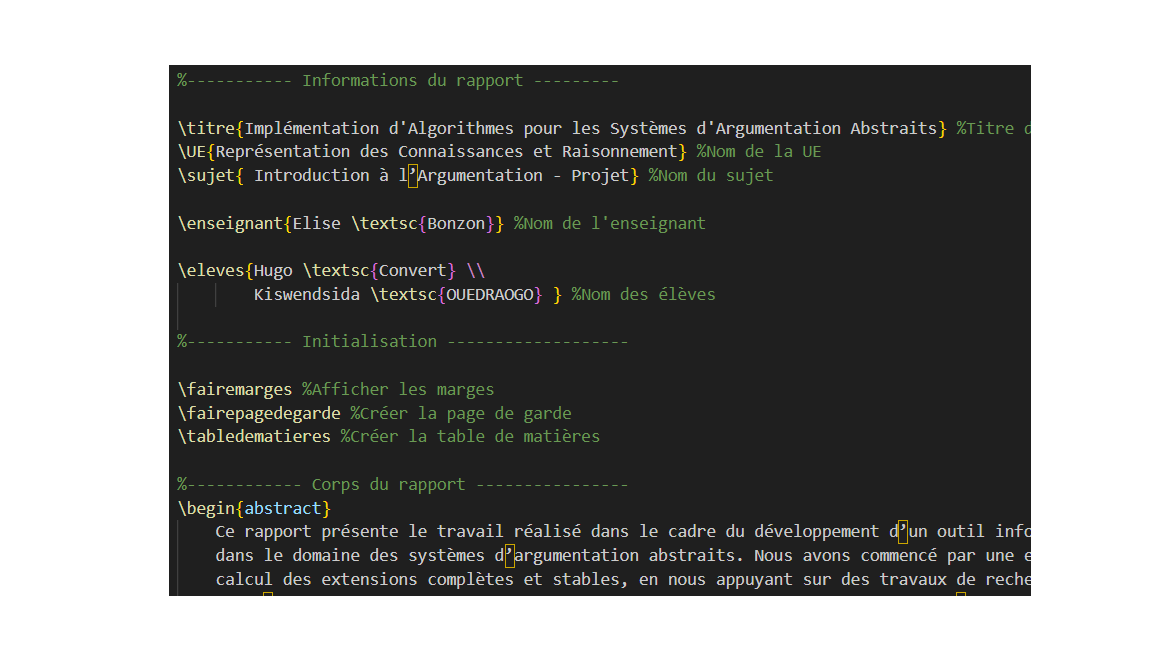
\includegraphics[width=\linewidth]{img/console_af1.png} \\[0.2cm]
		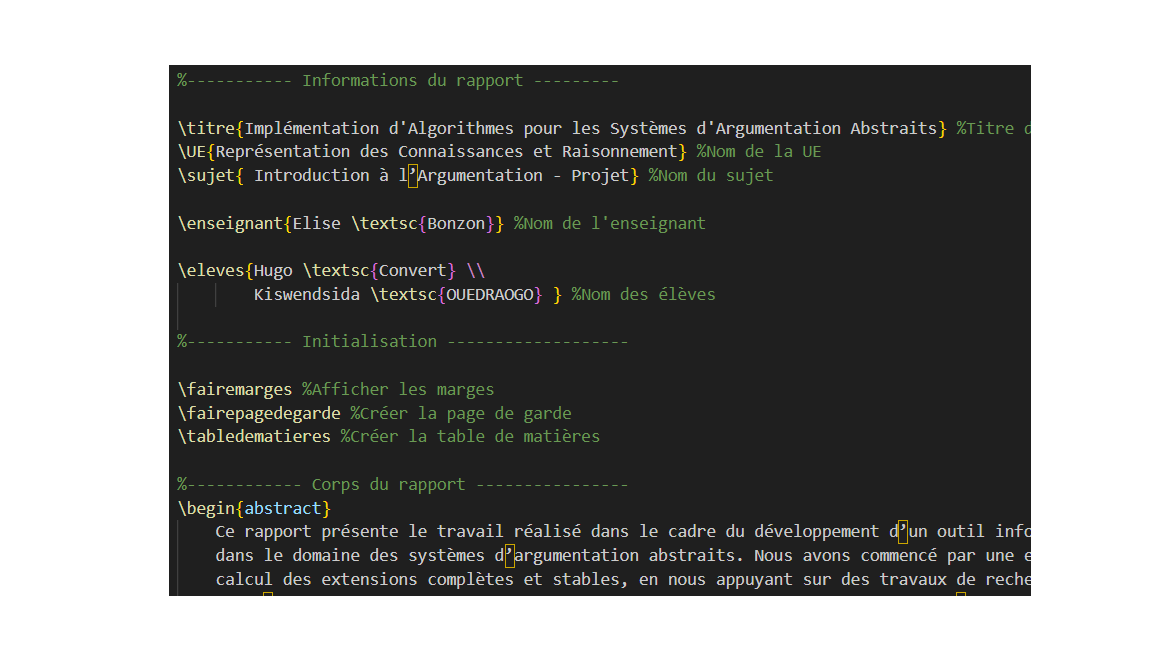
\includegraphics[width=\linewidth]{img/console_af1.png}
	\end{minipage} \\[0.2cm]


	
	\hline
	\texttt{python main.py -p SE-} & 
	\begin{itemize}
		\item Capture de la sortie console.
		\item Capture de l'interface graphique.
	\end{itemize} \\
	\hline
	\texttt{python main.py } & 
	\begin{itemize}
		\item Capture de la sortie console.
		\item Capture de l'interface graphique.
	\end{itemize} \\
	\hline
	\texttt{python main.py -p DS-SE -f ./tests/af4.apx -a arg3} & 
	\begin{itemize}
		\item Capture de la sortie console.
		\item Capture de l'interface graphique.
	\end{itemize} \\
	\hline
	\texttt{python main.py -p DC-SE -f ./tests/af4.apx -a arg3} & 
	\begin{itemize}
		\item Capture de la sortie console.
		\item Capture de l'interface graphique.
	\end{itemize} \\
	\hline
	\texttt{python main.py -p DC-SE -f ./tests/af5.apx -a arg3} & 
	\begin{itemize}
		\item Capture de la sortie console.
		\item Capture de l'interface graphique.
	\end{itemize} \\

	\end{longtable}




\vspace{0.5cm}
\noindent
Les résultats obtenus confirment le bon fonctionnement de notre implémentation des algorithmes. Les extensions calculées correspondent aux attentes théoriques pour chaque cas testé, validant ainsi l'exactitude de notre implémentation.


\section*{Conclusion}
En conclusion, ce projet a été l'occasion d'élargir nos connaissances sur les systèmes d'argumentation abstraits, 
à travers une revue de littérature et l'implémentation pratique d'algorithmes d'énumération des extensions. 

L'intégration de ces algorithmes dans un outil fonctionnel a permis de concrétiser nos apprentissages. 
Ce travail constitue une contribution significative à l'application des théories de l'argumentation et ouvre la voie à des perspectives d'amélioration.



\bibliographystyle{unsrt} 
\bibliography{mybib}

\end{document}
